\begin{appendix} 
\chapter{Characterization of the Human Body Lower Limb} \label{appendixA}
\section{Stacked Clustered Bar Charts}
This appendix presents the compiled data from the reviewed gait analysis studies in the form of charts, as the ones presented in \Cref{sec:characterizationKKP}, for the hip, knee and ankle joints. The parameters of torque, angle and power, were extracted.

\begin{figure}[htbp]
\centering
    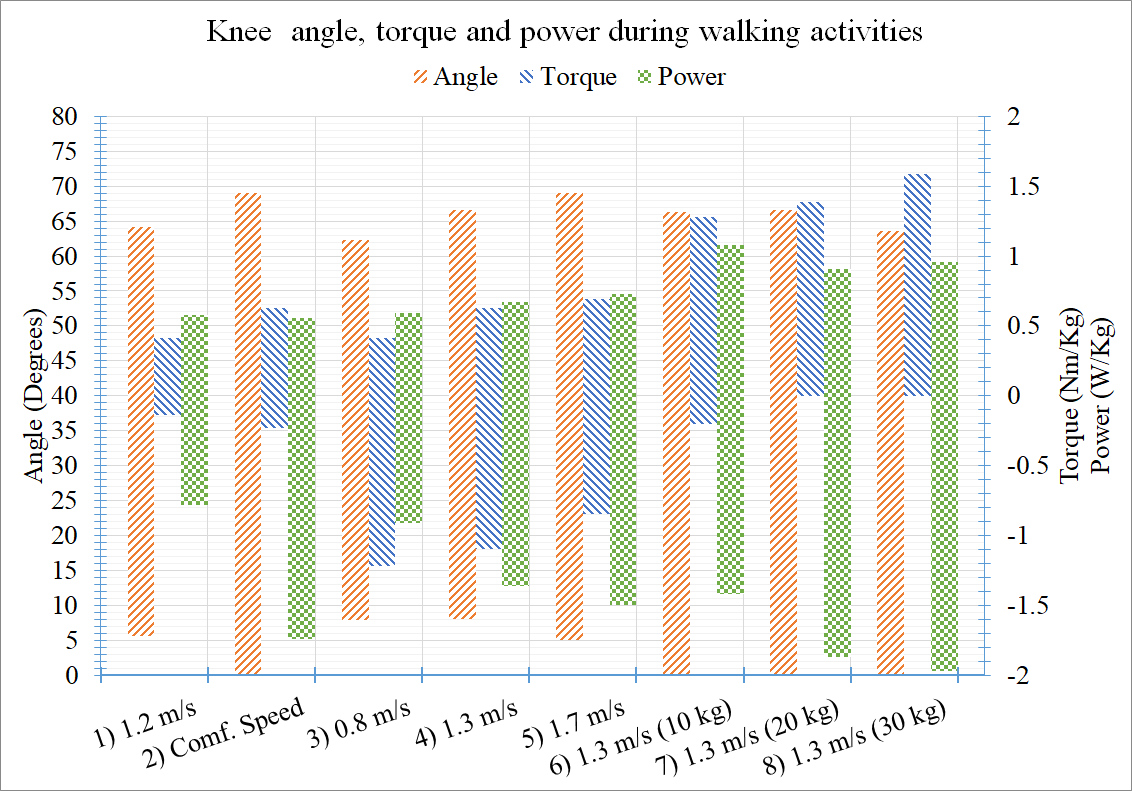
\includegraphics[width=\textwidth]{KneeKKPWalkingExcel.png}
    \caption{Data compiled from several experiments of the knee joint for walking over ground activities. The weight next to the name of some activities dictates the load carried by the subjects during the experiment. The torque and power are presented in the same axis since their values share the  same order of magnitude \cite{solis2017characterization}. The gait analysis studies are as follows: (1) \cite{bovi2011multiple}, (2) \cite{lee2008biomechanics}, (3-8) \cite{han2011biomechanical}.}
    \label{fig:kneeKKPWalking}
\end{figure}

\begin{figure}[htbp]
\centering
    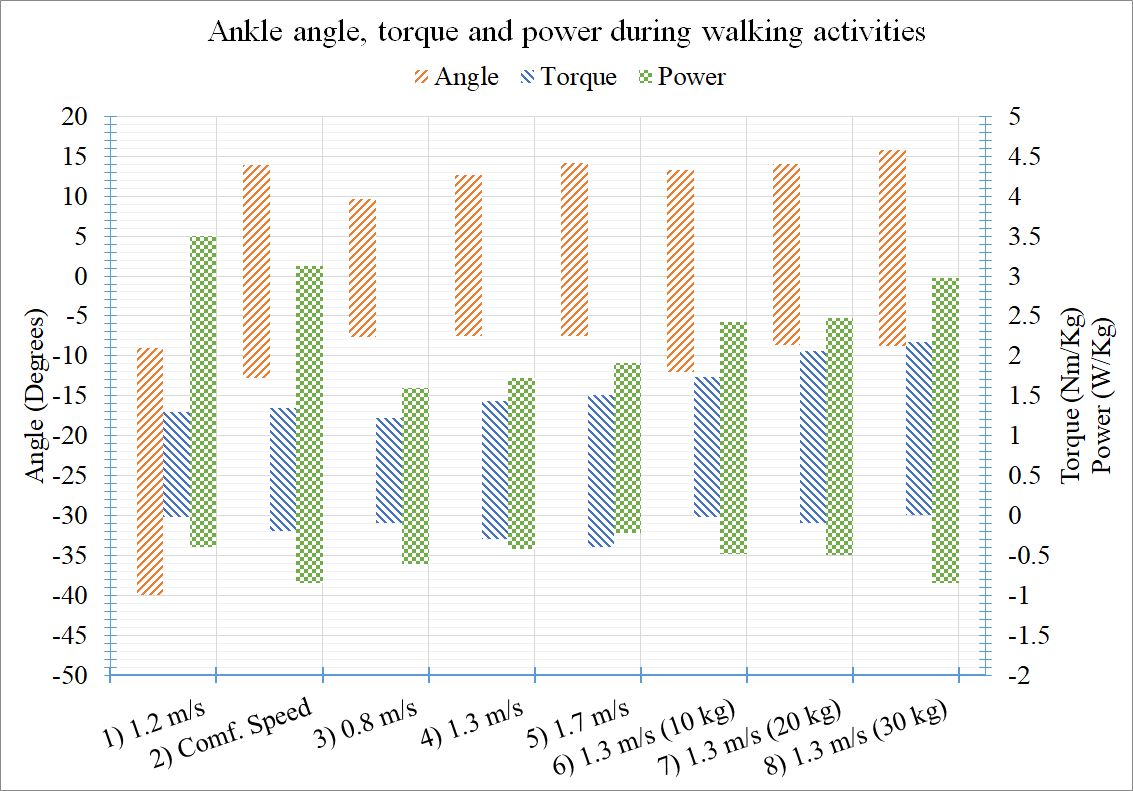
\includegraphics[width=\textwidth]{AnkleKKPWalkingExcel.png}
    \caption{Data compiled from several experiments of the ankle joint for walking over ground activities. The weight next to the name of some activities dictates the load carried by the subjects during the experiment. The torque and power are presented in the same axis since their values share the  same order of magnitude \cite{solis2017characterization}. The gait analysis studies are as follows: (1) \cite{bovi2011multiple}, (2) \cite{lee2008biomechanics}, (3-8) \cite{han2011biomechanical}.}
    \label{fig:ankleKKPWalking}
\end{figure}

\begin{figure}[htbp]
    \centering
    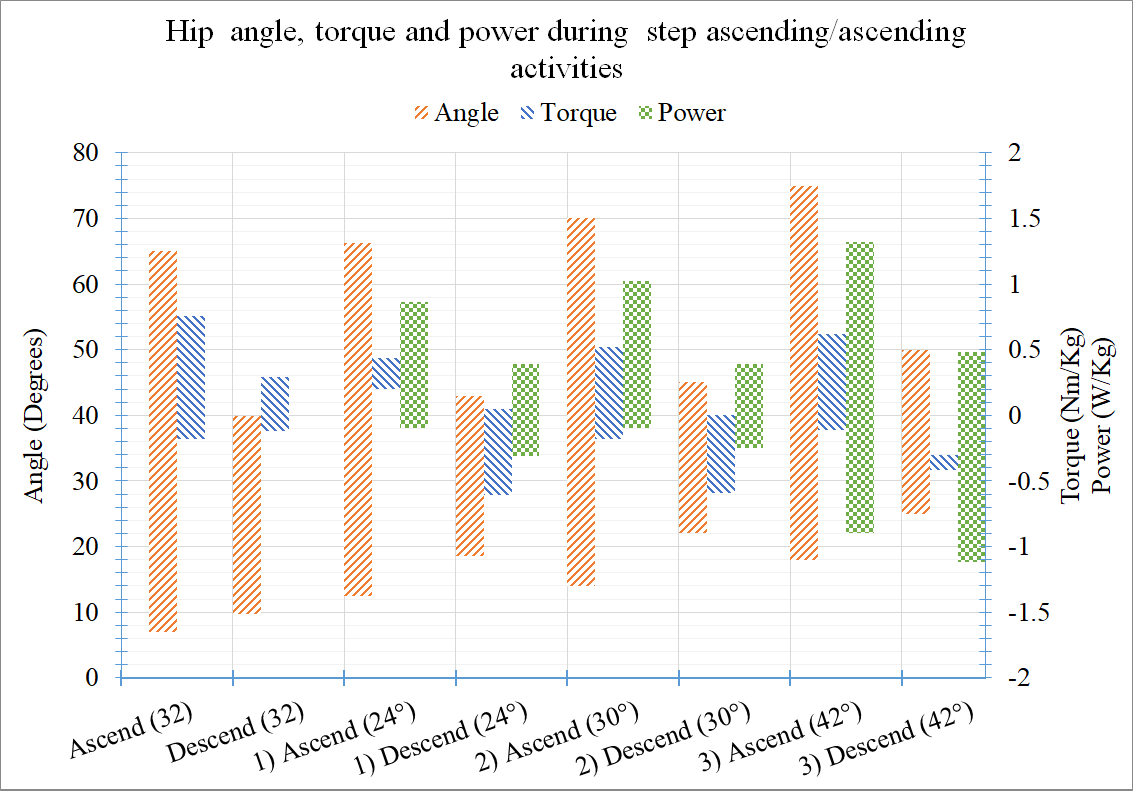
\includegraphics[width=\textwidth]{HipKKPStairsExcel.png}
    \caption{Data compiled from several experiments of the hip joint for stairs ascending/descending experiments. The weight next to the name of some activities dictates the load carried by the subjects during the experiment. The torque and power are presented in the same axis since their values share the  same order of magnitude \cite{solis2017characterization}. The gait analysis studies are as follows: (1) \cite{bovi2011multiple}, (2) \cite{lee2008biomechanics}, (3-8) \cite{han2011biomechanical}. }
    \label{fig:hipKKPStairs}
\end{figure}

\begin{figure}[htbp]
    \centering
    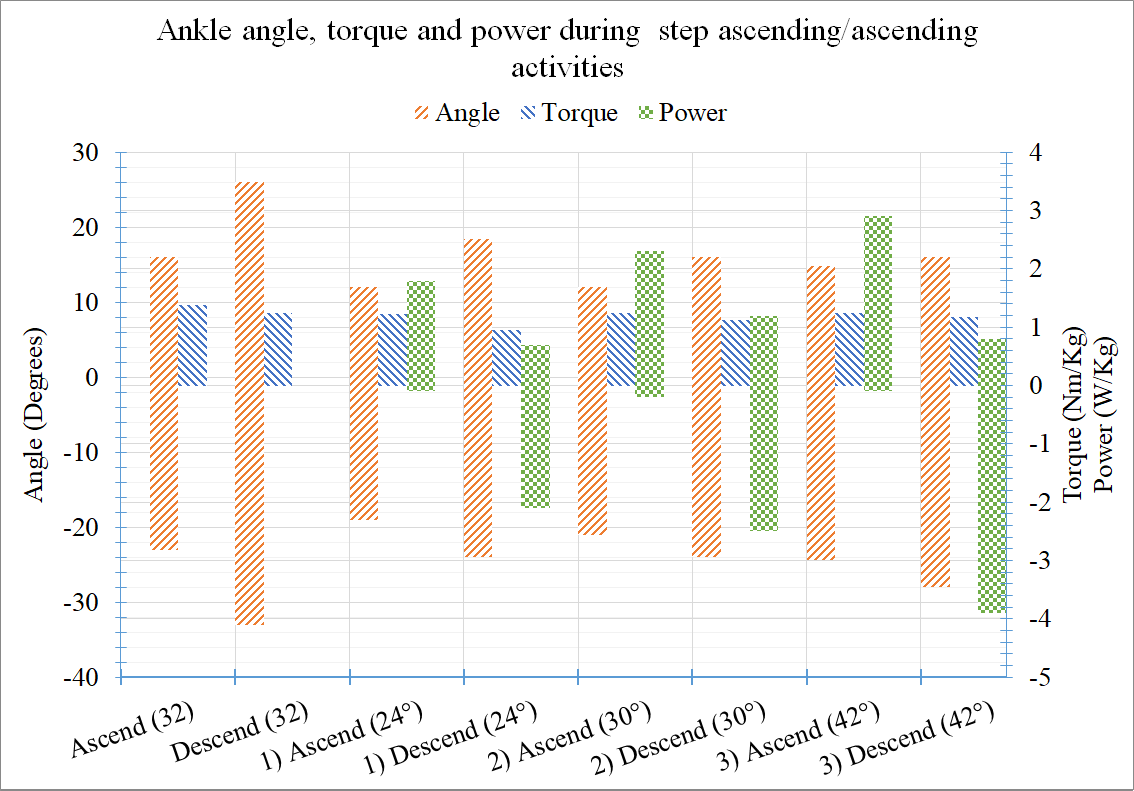
\includegraphics[width=\textwidth]{AnkleKKPStairsExcel.png}
    \caption{Data compiled from several experiments of the ankle joint for stairs ascending/descending experiments. The weight next to the name of some activities dictates the load carried by the subjects during the experiment. The torque and power are presented in the same axis since their values share the  same order of magnitude \cite{solis2017characterization}. The gait analysis studies are as follows: (1) \cite{bovi2011multiple}, (2) \cite{lee2008biomechanics}, (3-8) \cite{han2011biomechanical}. }
    \label{fig:ankleKKPStairs}
\end{figure}

\begin{figure}[htbp]
    \centering
    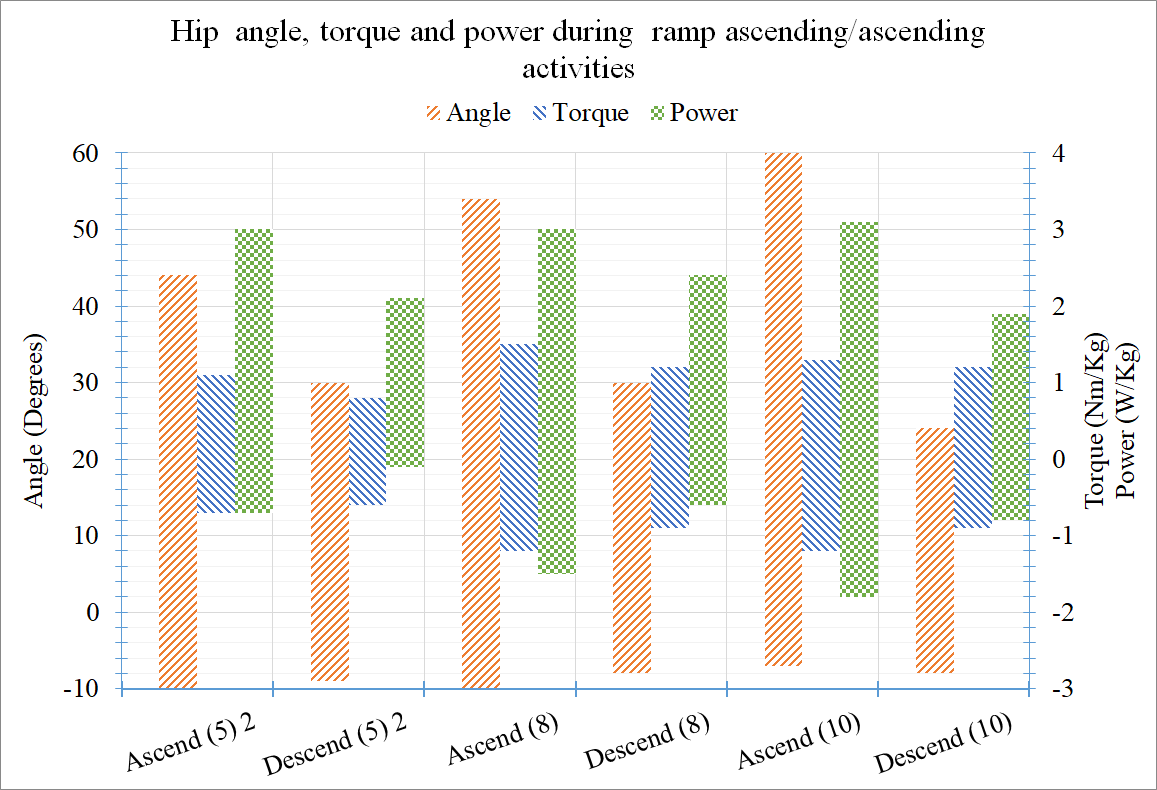
\includegraphics[width=\textwidth]{HipKKPRampExcel.png}
    \caption{Data compiled from several experiments of the hip joint for ramp ascending/descending experiments. UPDATE THIS: The weight next to the name of some activities dictates the load carried by the subjects during the experiment. The torque and power are presented in the same axis since their values share the  same order of magnitude \cite{solis2017characterization}. The gait analysis studies are as follows: (1) \cite{bovi2011multiple}, (2) \cite{lee2008biomechanics}, (3-8) \cite{han2011biomechanical}. }
    \label{fig:hipKKPRamp}
\end{figure}

\begin{figure}[htbp]
    \centering
    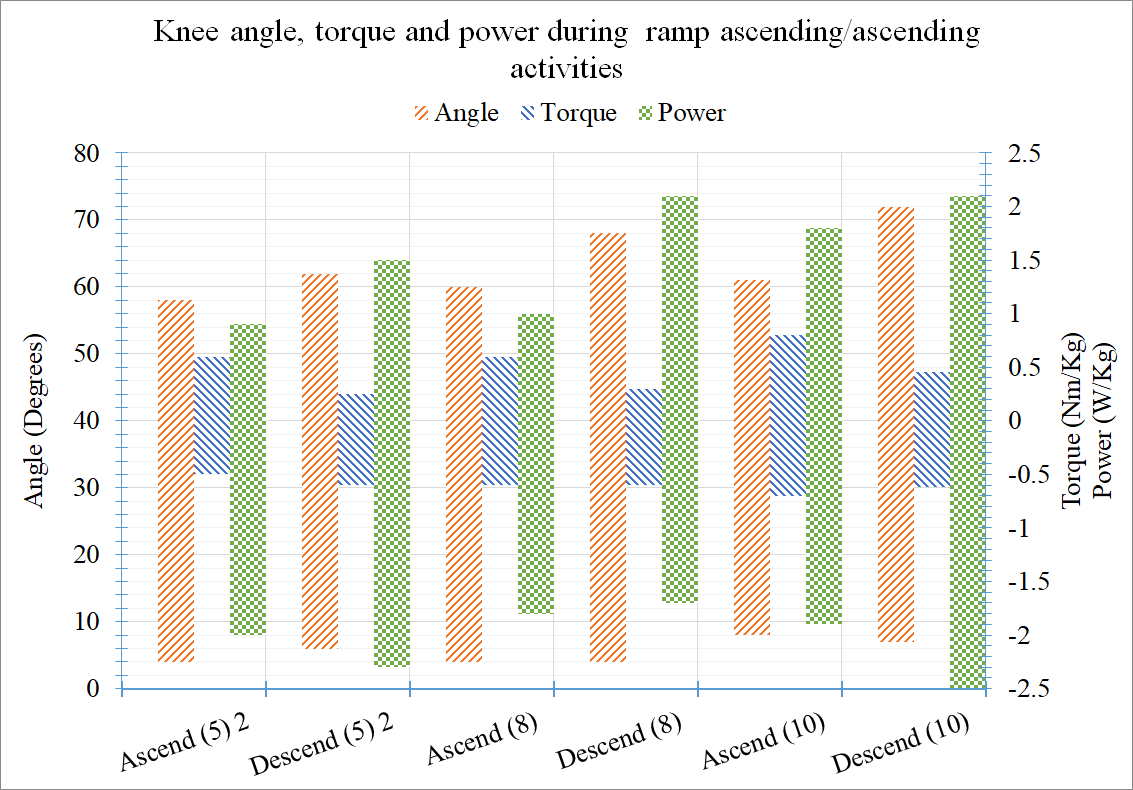
\includegraphics[width=\textwidth]{KneeKKPRampExcel.png}
    \caption{Data compiled from several experiments of the knee joint for ramp ascending/descending experiments. UPDATE THIS: The weight next to the name of some activities dictates the load carried by the subjects during the experiment. The torque and power are presented in the same axis since their values share the  same order of magnitude \cite{solis2017characterization}. The gait analysis studies are as follows: (1) \cite{bovi2011multiple}, (2) \cite{lee2008biomechanics}, (3-8) \cite{han2011biomechanical}. }
    \label{fig:kneeKKPRamp}
\end{figure}

\begin{figure}[htbp]
    \centering
    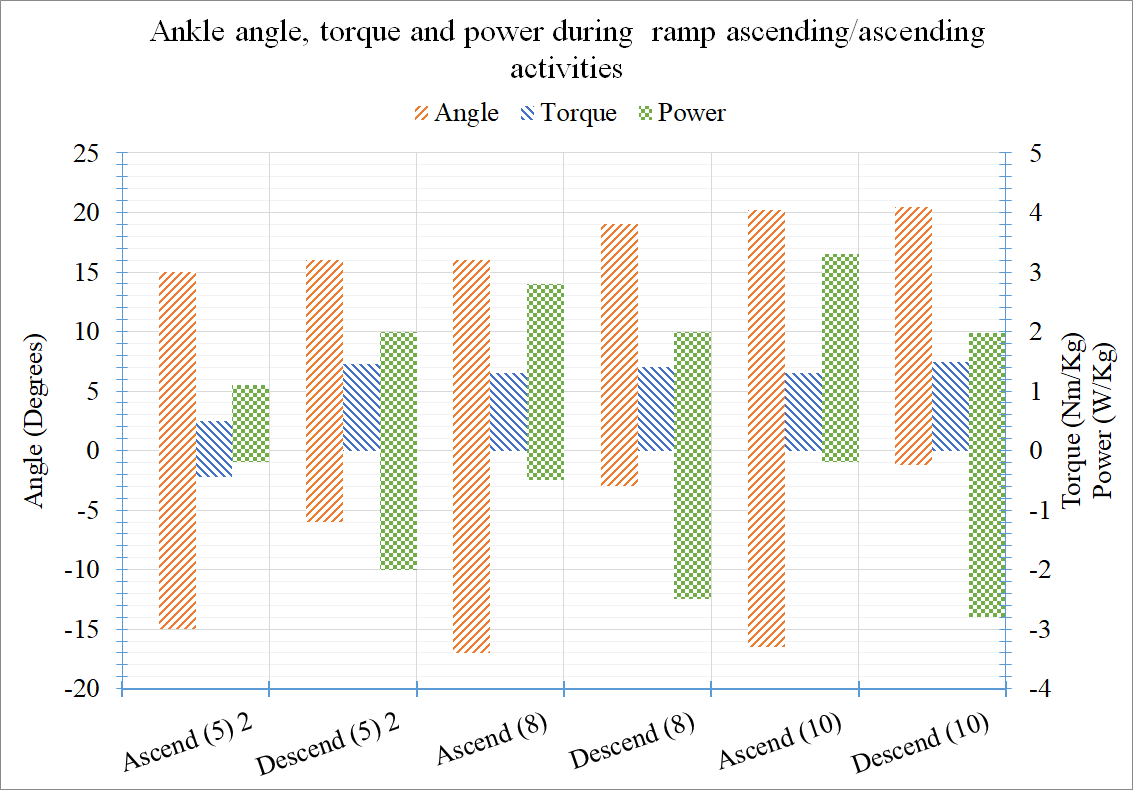
\includegraphics[width=\textwidth]{AnkleKKPRampExcel.png}
    \caption{Data compiled from several experiments of the ankle joint for ramp ascending/descending experiments. UPDATE THIS: The weight next to the name of some activities dictates the load carried by the subjects during the experiment. The torque and power are presented in the same axis since their values share the  same order of magnitude \cite{solis2017characterization}. The gait analysis studies are as follows: (1) \cite{bovi2011multiple}, (2) \cite{lee2008biomechanics}, (3-8) \cite{han2011biomechanical}. }
    \label{fig:ankleKKPRamp}
\end{figure}

\begin{figure}[htbp]
    \centering
    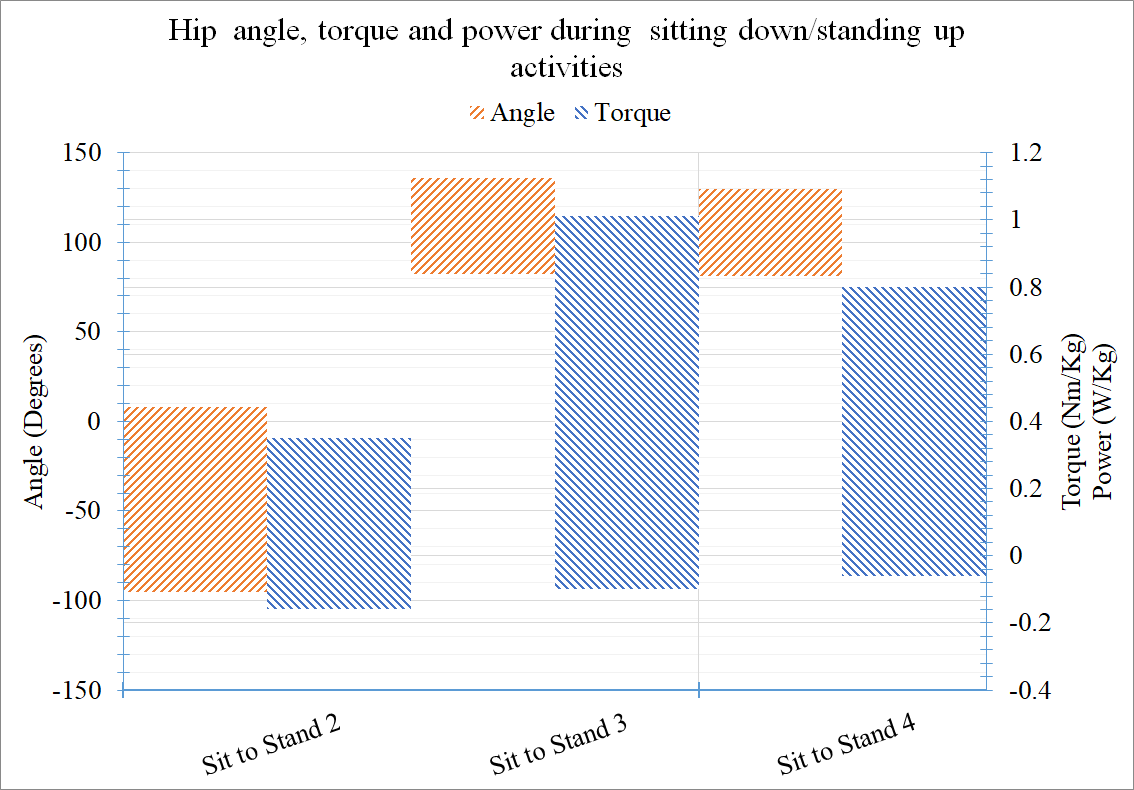
\includegraphics[width=\textwidth]{HipKKPSitExcel.png}
    \caption{Data compiled from several experiments of the hip joint for sit to stand/stand to sit experiments. UPDATE THIS: The weight next to the name of some activities dictates the load carried by the subjects during the experiment. The torque and power are presented in the same axis since their values share the  same order of magnitude \cite{solis2017characterization}. The gait analysis studies are as follows: (1) \cite{bovi2011multiple}, (2) \cite{lee2008biomechanics}, (3-8) \cite{han2011biomechanical}.  }
    \label{fig:hipKKPSit}
\end{figure}

\begin{figure}[htbp]
    \centering
    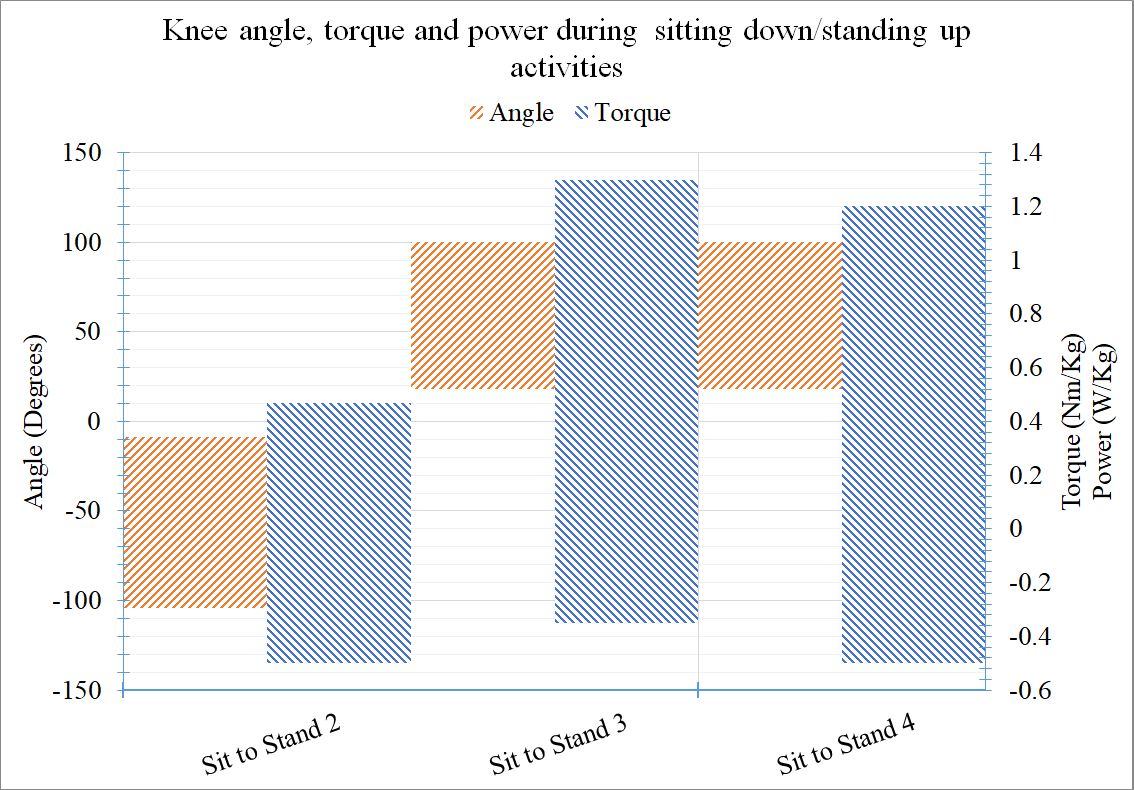
\includegraphics[width=\textwidth]{KneeKKPSitExcel.png}
    \caption{Data compiled from several experiments of the knee joint for sit to stand/stand to sit experiments. UPDATE THIS: The weight next to the name of some activities dictates the load carried by the subjects during the experiment. The torque and power are presented in the same axis since their values share the  same order of magnitude \cite{solis2017characterization}. The gait analysis studies are as follows: (1) \cite{bovi2011multiple}, (2) \cite{lee2008biomechanics}, (3-8) \cite{han2011biomechanical}. }
    \label{fig:kneeKKPSit}
\end{figure}

\begin{figure}[htbp]
    \centering
    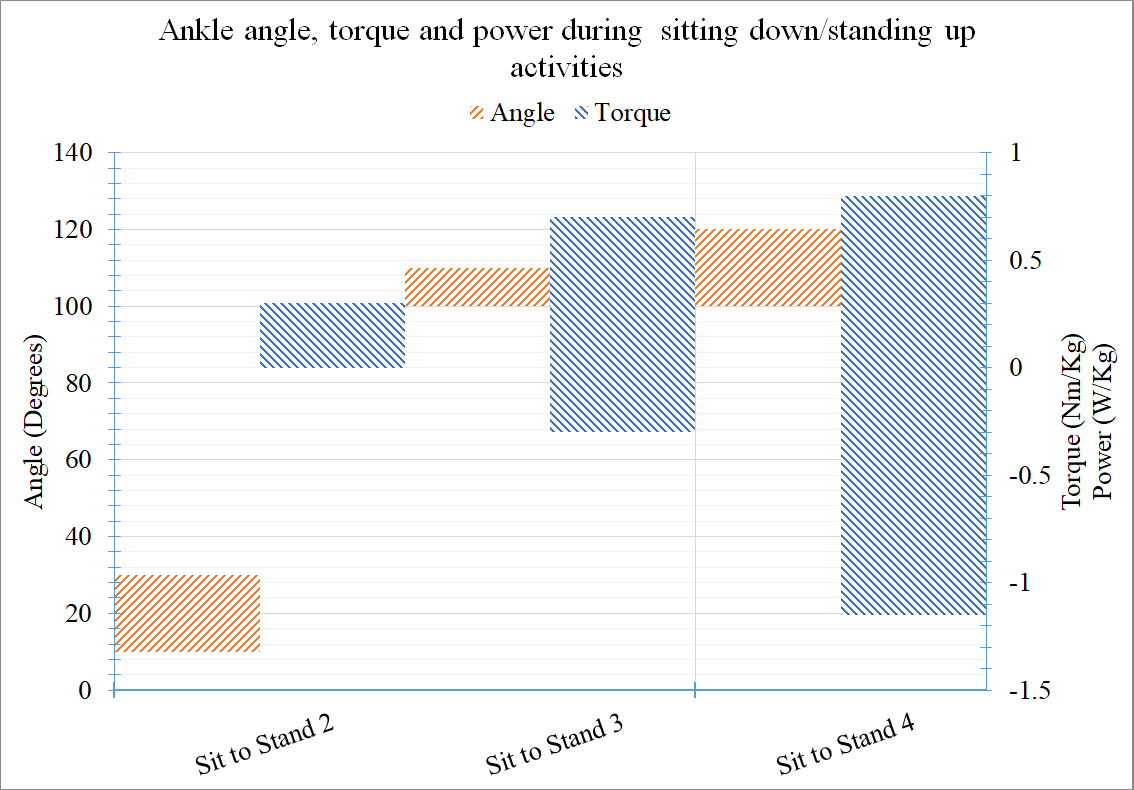
\includegraphics[width=\textwidth]{AnkleKKPSitExcel.png}
    \caption{Data compiled from several experiments of the ankle joint for sit to stand/stand to sit experiments. UPDATE THIS: The weight next to the name of some activities dictates the load carried by the subjects during the experiment. The torque and power are presented in the same axis since their values share the  same order of magnitude \cite{solis2017characterization}. The gait analysis studies are as follows: (1) \cite{bovi2011multiple}, (2) \cite{lee2008biomechanics}, (3-8) \cite{han2011biomechanical}. }
    \label{fig:ankleKKPSit}
\end{figure}

\end{appendix}
